\documentclass[12pt,english,a4paper]{article}
\usepackage[utf8]{inputenc}
\usepackage[T1]{fontenc}
\usepackage{babel,amsmath,amsthm,graphicx,mathtools,textcomp,varioref,amssymb,float,listings}
\usepackage[top=50pt,left=40pt,right=40pt]{geometry}
\usepackage{titling,wrapfig}
\usepackage{color}
\usepackage{csquotes}
\usepackage{verbatim}
\usepackage{csvsimple}
\usepackage{booktabs}
\usepackage[
backend=biber,
style=alphabetic,
citestyle=authoryear,
sorting=nyt
]{biblatex}
\addbibresource{bibliography.bib}
 
 
\definecolor{codegreen}{rgb}{0,0.6,0}
\definecolor{codegray}{rgb}{0.5,0.5,0.5}
\definecolor{codepurple}{rgb}{0.58,0,0.82}
\definecolor{backcolour}{rgb}{0.95,0.95,0.92}
 
\lstdefinestyle{mystyle}{
    backgroundcolor=\color{backcolour},   
    commentstyle=\color{codegreen},
    keywordstyle=\color{magenta},
    numberstyle=\tiny\color{codegray},
    stringstyle=\color{codepurple},
    basicstyle=\footnotesize,
    breakatwhitespace=false,         
    breaklines=true,                 
    captionpos=b,                    
    keepspaces=true,                 
    numbers=left,                    
    numbersep=5pt,                  
    showspaces=false,                
    showstringspaces=false,
    showtabs=false,                  
    tabsize=2
}
 
\lstset{style=mystyle}


\let\vecarrow\vec
\renewcommand{\vec}[1]{\mathbf{#1}}
\let\oldhat\hat
\renewcommand{\hat}[1]{\oldhat{\mathbf{#1}}}
\def\doubleunderline#1{\underline{\underline{#1}}}
\linespread{1.6}
\renewcommand{\qedsymbol}{$\blacksquare$}

\let\~\tilde

\newcommand{\justdiff}[1]{\frac{\partial}{\partial#1}}
\newcommand{\pdiff}[2]{\frac{\partial #1}{\partial#2}}
\newcommand{\ppdiff}[2]{\frac{\partial^2 #1}{\partial#2^2}}
\newcommand{\proofsquare}{\begin{proof}[] \end{proof}}
\let\f\frac
\DeclareMathOperator{\arccosh}{arcosh}

\DeclarePairedDelimiter\abs{\lvert}{\rvert}%
\DeclarePairedDelimiter\norm{\lVert}{\rVert}%

\makeatletter
\csvset{
  autobooktabularcenter/.style={
    file=#1,
    after head=\csv@pretable\begin{tabular}{*{\csv@columncount}{l}}\csv@tablehead,
    table head=\toprule\csvlinetotablerow\\\midrule,
    late after line=\\\midrule,
    table foot=\\\bottomrule,
    late after last line=\csv@tablefoot\end{tabular}\csv@posttable,
    command=\csvlinetotablerow},
}
\makeatother
\newcommand{\csvautotabularcenter}[2][]{\csvloop{autotabularcenter={#2},#1}}
\newcommand{\csvautobooktabularcenter}[2][]{\csvloop{autobooktabularcenter={#2},#1}}

\tolerance = 5000
\hbadness = \tolerance
\pretolerance = 2000

\title{FYS4150: Project 3}
\author{Jonathan Brakstad Waters\\Øyvind Engebretsen Elgvin\\Henrik Lind Petlund}

\begin{document}

\begin{titlepage}
\maketitle
\begin{abstract}
    
\end{abstract}

\end{titlepage}

\section{Introduction} \label{introduction}

The Ising model is a model that has a large variety of usage. In this report, the model will be used to study phase transitions and thermodynamic properties in magnetic systems. The systems at hand are systems of size $L\times L$ particles in a grid. Each particle may be in either state "up" or "down" denoted with $1$ and $-1$, respectively. The model only focuses on the interaction between the nearest neighbor particles, and the energy between these is given by
\begin{align}
    E = -J \sum_{<kl>}^N s_ks_l 
\end{align}
where $N$ is the number of particles, $s_i=\pm 1$ and $J>0$ is a constant which represents ferromagnetism and the strength of the particle interactions. We assume periodic boundary conditions so that every particle in the lattice has four nearest neighbors. 

Further, the partition function of the system is given by
\begin{equation}
Z=\sum_i e^{-\beta E_i} \label{eq:partition}
\end{equation}
the specific heat capacity
\begin{equation}
C_V=\frac{1}{k_B T^2}\left(\langle E^2\rangle-\langle E\rangle^2\right)
\end{equation}
the magnetisation
\begin{equation}
M=\sum_is_i
\end{equation}
and the susceptibility
\begin{equation}
\chi= \frac{1}{k_B T}\left(\langle M^2\rangle-\langle M\rangle^2\right)
\end{equation}
as functions of the energy and spin. Where, $\beta =1/k_B T$. These equations are also mentioned in the lecture slides by (\cite{LectureIsing}) from the course FYS3150.

Initially, we will derive values of a 2x2 case and thereafter, proceed to higher dimensions. In a higher dimension case with $L=20$, the time it takes to reach the most likely state, represented by the number of Monte Carlo cycles, is calculated for two different temperatures with both an ordered and a random initial state. This gives an estimate of the equilibrium time of the system. The energy data from this case is then translated to a probability function $P(E)$. 

Next, the systems with $L=40, L=60, L=80$ and $L=100$ are studied as functions of temperature. These calculations are performed to try and simulate phase transitions in the systems. For successfully detected phase transitions, the critic temperature is also extracted and compared to the exact.

\section{Methods and theory} \label{methods_and_theory}

\subsection{Benchmarks}

For the $2x2$ case, the energy, magnetic momentum, specific heat capacity, and the magnetic susceptibility can all be calculated analytically. These analytical values, shown in Table \ref{tab:benchmarks}, are used as benchmarks for the numerically derived values.

\subsection{The Metropolis algorithm}

The heavy calculation in this project is done by the \textit{metropolis} algorithm. The steps of this algorithm are:

1. Initialize a random initial state with the energy $E_0$. This state will have spins in random directions. 

2. Choose a random spin particle in the lattice, and flip it.

3. Calculate the energy change, $\Delta E=E_1-E_0$, caused by the flipped spin. If $\Delta E \le 0$, the spin change is accepted, and step 6 is the next step.

4. If the $\Delta E > 0$, calculate the the Boltzmann distribution $w=e^{-\beta \Delta E}$.

5. Calculate a random number $r$. If $r \le w$, the new configuration is accepted, otherwise the old configuration is kept.

6. Update the expectation values (energy, magnetization, heat capacity, and susceptibility).

7. Repeat steps 2-6 until the values are satisfying.


\noindent Step 2-6 is what is called a Monte Carlo cycle and is, in turn, a measurement of the energy of the system. The final values are to be divided by the total number of Monte Carlo cycles used. The Metropolis algorithm is described more thoroughly in the lecture notes of FYS3150 (\cite{LectureIsing}) with code examples.

\subsection{Periodic boundary conditions}
To account for the fact that some of the spins at the boundary of the lattice does not have four nearest neighbours, periodic boundary conditions are introduced. This means that a spin at a boundary i.e. $s_{N,0}$ has a neighbour to the right with the same spin as the particle $s_{0,0}$. In one dimension, this can be expressed by
\begin{align*}
    E_i=-J\sum_{j=1}^{N}s_js_{j+1}
\end{align*}

\noindent For small dimensions, the energy of the system will be significantly affected by whether or not periodic boundary conditions are implemented. As $N \rightarrow \infty$, the boundary becomes insignificant. This is what happens when looking at phase transitions and critical temperatures, where the system has to be described in a larger dimension.

\subsection{Phase transitions}
In the Ising model, it is interesting to see if it is possible to estimate phase transitions in the systems. These phase transitions can be i.e. liquid/gas (first order) or ferromagnetic/paramagnetic (second order). These transitions are all depending on the parameter, $T_C$, called the Curie temperature or the critical temperature. The theory given in the Lecture notes of FYS3150 (\cite{LectureIsing}) can be used to describe some of the values in the Ising model class with a power law behavior as follows
\begin{equation}
    \langle M(T)\rangle\sim (T-T_c)^\beta \propto L^{-\beta/\nu}
\end{equation}
\begin{equation}
    C_V(T)\sim (T-T_c)^{-\gamma} \propto L^{-\alpha/\nu}
\end{equation}
\begin{equation}
    \chi(T)\sim (T-T_c)^\alpha \propto L^{-\gamma/\nu}
\end{equation}
where $\beta = 1/8$ is the so called critical exponent, $\alpha = 0$ and $\gamma = 7/4$. The value of $\nu$ is defined by the correlation length which has a divergent behavior when approaching $T_c$
\begin{equation}
      \xi(T) \propto L \sim \left|T_C-T\right|^{-\nu},
  \label{eq:xi}
\end{equation}

\noindent The lattice sizes in this report are always finite, and therefore $\chi$ will be proportional to this lattice size as seen in the equations above. Using finite size scaling relations, it is possible to relate the results and behaviors in the finite lattices with the once from the infinite case. This results in a scaling of the critical temperature given by

\begin{equation}
    T_C(L)-T_C(L=\infty) = aL^{-1/\nu} \label{eq:tc}
\end{equation}
with $\nu = 1$. The exact result for $T_c(L=\infty)$ is found in (\cite{LarsOns}), and is given as the dimensionless value
\begin{align*}
    kT_c/J=\frac{2}{ln(1+\sqrt{2})}=2.269
\end{align*}
If a phase transition is observed in a finite system, the critical temperature, $T_{c}(L_i)$, is possible to derive. The value of $T_{c}(L=\infty)$ can be derived if one has two temperatures from finite systems by using \eqref{eq:tc}. This would result in two equations with two unknown variables; $T_c(L=\infty)$ and $a$, given by
\begin{align*}
    \begin{cases}
        T_c(L=\infty)=T_c(L_1)-aL_1^{-1/\nu}\\
        T_c(L=\infty)=T_c(L_2)-aL_2^{-1/\nu}
    \end{cases}
\end{align*}
subtracting these and solving for $a$ results in
\begin{align*}
    a=\frac{T_c(L_1)-T_c(L_2)}{L_1^{-1/\nu}-L_2^{-1/\nu}}
\end{align*}
which reveals the expression for the critical temperature in a infinite system as
\begin{equation}
    T_c(L=\infty)=T_c(L_1)-\left(\frac{T_c(L_1)-T_c(L_2)}{L_1^{-1/\nu}-L_2^{-1/\nu}}\right)L_1^{-1/\nu}
    \label{eq:critical}
\end{equation}

\section{Results} \label{results}

\subsection{The 2x2 Case}

Table \ref{tab:configurations} lists the different possible spin configurations with their respective degeneracy, energy and magnetization in the 2x2 lattice, whereas Table \ref{tab:benchmarks} displays the analytic and experimental values of interest in the 2x2 lattice.

\begin{table}[H]
    \centerline{\csvautobooktabularcenter{E_M_Configurations.csv}}
    \caption{List of the different possible spin configurations with their respective degeneracy, energy and magnetization in the 2x2 case.}
    \label{tab:configurations}
\end{table}

\begin{table}[H]
    \centerline{\csvautobooktabular{Benchmarks.csv}}
    \caption{List of analytical and experimental values for the $2x2$ lattice with the absolute relative deviation. All values are scaled by the number of spin ($L^2$).}
    \label{tab:benchmarks}
\end{table}

\subsection{The most likely state}

Figure \ref{fig:E_equiv} and Figure \ref{fig:M_equiv} gives a graphical presentation of the time ($\#$ of MC-cycles) it takes for different systems to reach equilibrium. Depending on the ordering of the initial state and the temperature of the different systems; an estimate of the equilibrium time can be made. Figure \ref{fig:acc_conf} gives the number of accepted configurations as function of MC-cycles.

\begin{figure}[H]
    \centering
    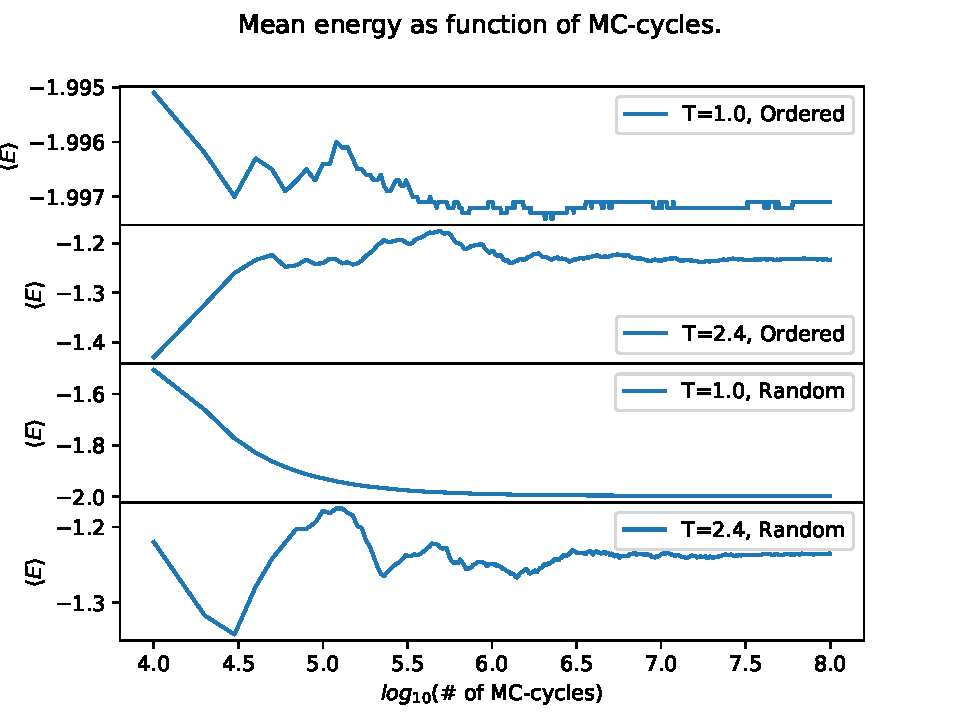
\includegraphics[scale=0.7]{Code_Files/Figures/Most_Likely_State_E_mean_L_20.pdf}
    \caption{The mean energy for temperatures $T=[1.0,2.4]$ in both an ordered and random initial state as function of MC-cycles (time), L = 20. The x-axis is logarithmically scaled and there are $10^4$ MC-cycles between each data point.}
    \label{fig:E_equiv}
\end{figure}
\begin{figure}[H]
    \centering
    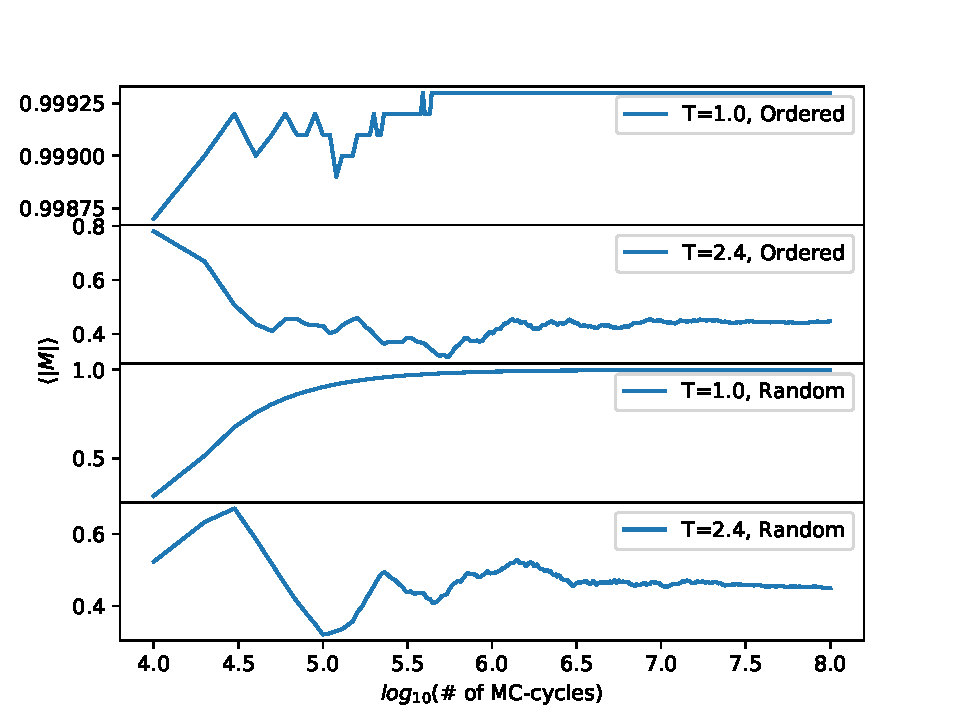
\includegraphics[scale=0.7]{Code_Files/Figures/Most_Likely_State_M_abs_L_20.pdf}
    \caption{The mean absolute magnetization for temperatures $T=[1.0,2.4]$ in both an ordered and random initial state as function of MC-cycles (time), L = 20. The x-axis is logarithmically scaled and there are $10^4$ MC-cycles between each data point.}
    \label{fig:M_equiv}
\end{figure}
\begin{figure}[H]
    \centering
    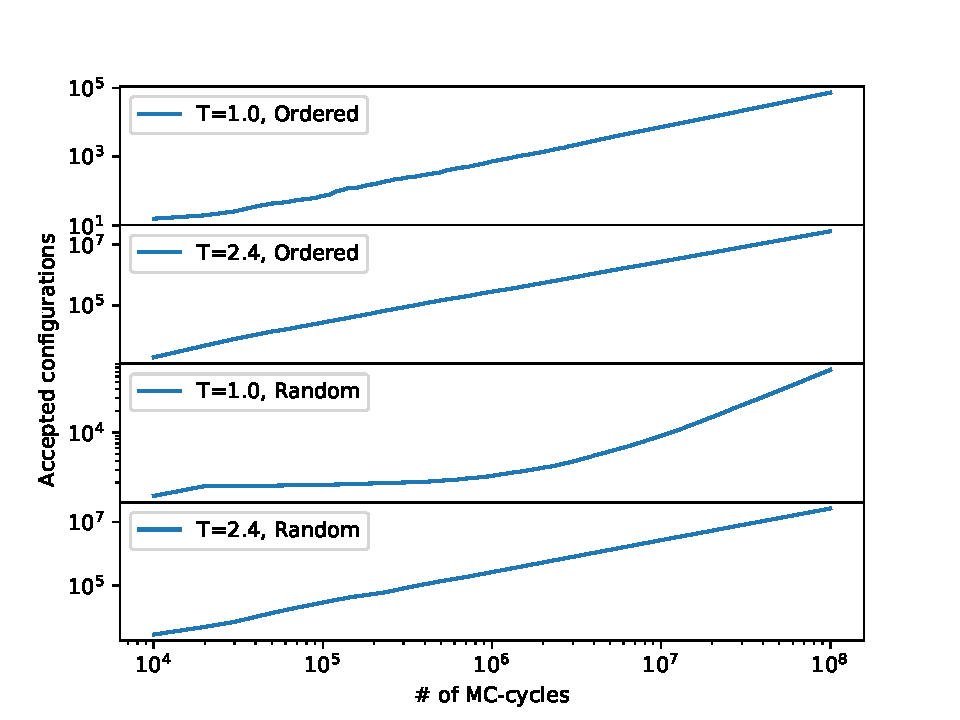
\includegraphics[scale=0.7]{Code_Files/Figures/Number_of_Accepted_Configs_L_20.pdf}
    \caption{Number of accepted configurations for temperatures $T=[1.0,2.4]$ in both an ordered and random initial state as function of MC-cycles (time), L = 20 presented in a loglog plot. There are $10^4$ MC-cycles between each data point.}
    \label{fig:acc_conf}
\end{figure}

\subsection{The Probability Distribution}

Her trenger vi kun fire plot av de tilhørende probability distributions plottene til de forrige resultatene. Det kan her også være kult å innlemme $\sigma _E^2$ i plottet i form av standardavviket fra mean-verdien. For eksempel slik som fra wikipedia: \url{https://en.wikipedia.org/wiki/File:Comparison_standard_deviations.svg}.

\begin{figure}[H]
    \centering
    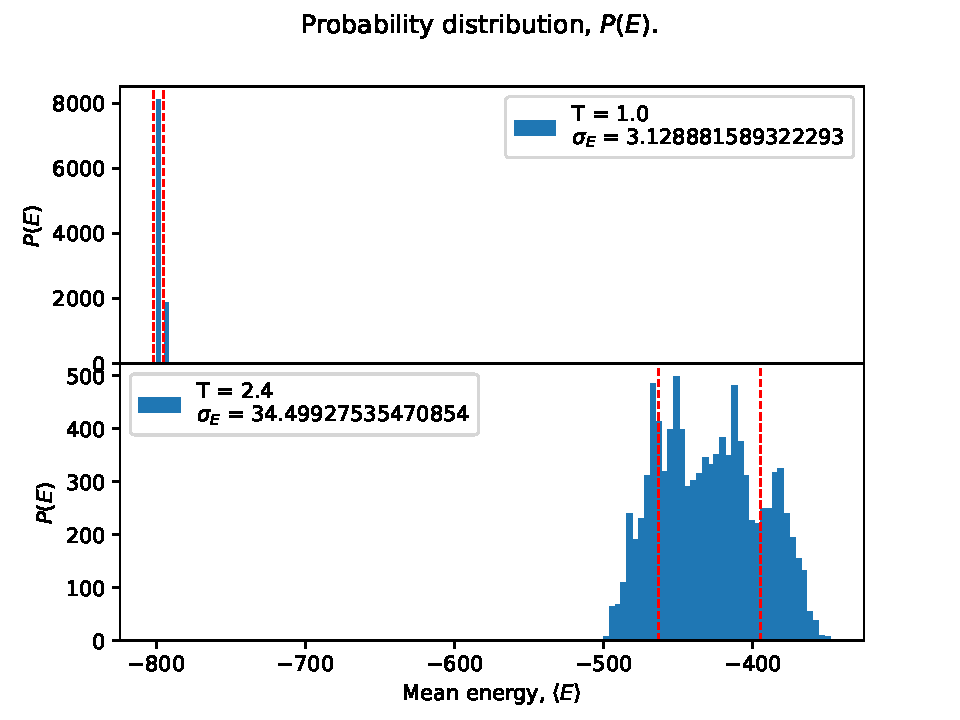
\includegraphics[scale=0.7]{Code_Files/Figures/Probability_Distribution_N_1000000000_L_20.pdf}
    \caption{Probability distribution of the energy, $E$, in a lattice of size L = 20 for temperatures $T = [1.0,2.4]$. The data comes from $10^6$ energies that are collected after equilibrium has been reached. The red dashed lines shows the first order standard deviation, $\sigma_E$, from the mean energy.}
    \label{fig:probability}
\end{figure}

\subsection{Phase transitions and the critical temperature, $T_c$}

Figure \ref{fig:E_of_T}-\ref{fig:X_of_T} in section \ref{appendix} shows $\langle E\rangle$, $\langle |M|\rangle$, $C_v$ and $\chi_{abs}$ as function of temperature. From the $L=100$ curves, by the use of Equation \eqref{eq:critical}, the critical temperature of an infinite lattice is derived numerically. Table \ref{tab:critical} compares this to the one derived in \cite{LarsOns}. 

\begin{table}[H]
    \centerline{\csvautobooktabular{critical.csv}}
    \caption{Experimentally derived critical temperature, $T_c(L=\infty)$, compared to the exact temperature by \cite{LarsOns}.}
    \label{tab:critical}
\end{table}

\section{Discussion} \label{discussion}

Tenker vi kan kjøre samme struktur i denne seksjonen som i resultatseksjonen, slik at vi diskuterer hvert system/delopggave for seg.

\section{Conclusion} \label{conclusion}

\section{Appendix} \label{appendix}

\subsection{Calculating the benchmarks}

Finding the analytical values, we start by calculating the energies for the configurations of all possible spins. The number of configurations in the $2x2$ case is  $2^4 = 16$, in total. The energies are given by summing the interaction between the four neighbors
\begin{align*}
    E = -J \sum_{<kl>}^N s_ks_l 
\end{align*}
where an interaction is one of the four possible:
\begin{align*}
    E_{\uparrow \uparrow} = E_{\downarrow \downarrow} = -2J, 
\end{align*}
\begin{align*}
    E_{\uparrow \downarrow} = E_{\downarrow \uparrow} = 2J
\end{align*}
The $2x2$ case can then be divided in degeneracy of energies by how many spin up there is
\begin{align*}
    E_{\text{4 spin}\uparrow} = (-2J) + (-2J) + (-2J) + (-2J) = -8J \text{ with degeneracy = 1}
\end{align*}
\begin{align*}
    E_{\text{3 spin}\uparrow} = 2J + (-2J) + 2J + (-2J) = 0 \text{ with degeneracy = 4}
\end{align*}
\begin{align*}
    E_{\text{2 spin}\uparrow} = (-2J) + 2J + (-2J) + 2J = 0 \text{ with degeneracy = 4}
\end{align*}
\begin{align*}
    E_{\text{2 spin}\uparrow} = 2J + 2J + 2J + 2J = 8J \text{ with degeneracy = 2}
\end{align*}
\begin{align*}
    E_{\text{1 spin}\uparrow} = 2J + 2J + (-2J) + (-2J) = 0 \text{ with degeneracy = 4}
\end{align*}
\begin{align*}
    E_{\text{0 spin}\uparrow} = (-2J) + (-2J) + (-2J) + (-2J) = -8J \text{ with degeneracy = 1}
\end{align*}
with the associated magnetic moment, $M$, calculated for each spin configuration as
\begin{align*}
    M_{i}=\sum_{j=1}^{N} s_{j}
\end{align*}
as shown table 1.

With these energies, degeneracies, magnetization, and periodic boundary conditions we can calculate the analytical benchmark expressions, starting with the participation function, which is calculated as
\begin{align*}
    Z = \sum_{i=1}^{2^n} e^{-\beta E_i}
      = 2e^{\beta 8J} + 2e^{-\beta 8J} + 12
      = 4cosh(\beta 8J) + 12
\end{align*}
The expectation value for the energy
\begin{align*}
    <E> \hspace{0.2cm} 
        = \sum_{i=1}^{2^n} E_iP_i(T) 
        = \frac{1}{Z} \sum_{i=1}^{16} E_ie^{-\beta E_i}
        = - \frac{\delta ln(Z(T))}{\delta \beta}
        = -\frac{32sinh(\beta 8J)}{4cosh(\beta 8J) + 12}
\end{align*}
and the expression for the expectation value for the energy squared
\begin{align*}
    <E^2> \hspace{0.2cm} 
          = \sum_{i=1}^{2^n} E_i^2P_i(T) 
          = \frac{1}{Z} \sum_{i=1}^{16} E_i^2e^{-\beta E_i}
          = \frac{128J^2e^{\beta 8J} + 128J^2e^{-\beta 8J}}
                 {4cosh(\beta 8J) + 12}
          = \frac{64J^2cosh(\beta 8J)}{cosh(\beta 8J) + 3}
\end{align*}
The specific heat capacity take the expression
\begin{align*}
    C_v = \frac{\sigma_E^2}{k_BT^2} 
\end{align*}
where the variance, $\sigma_E^2$, is
\begin{align*}
    \sigma_E^2 = \hspace{0.2cm} <E^2> - <E>^2 \hspace{0.2cm}
               = \frac{64J^2cosh(\beta 8J)}{cosh(\beta 8J) + 3}
               - \bigg(-\frac{32sinh(\beta 8J)}{4cosh(\beta 8J) + 12}\bigg)^2
\end{align*}
Similarly, the analytic expressions of the magnetic moment are calculated as
\begin{align*}
    <M> \hspace{0.2cm} 
        = \sum_{i=1}^{2^n} M_iP_i(\beta) 
        = \frac{1}{Z} \sum_{i=1}^{16} M_ie^{-\beta E_i} = 0 
\end{align*}
and the mean absolute value of the magnetic moment is given by 
\begin{align*}
    <|M|> \hspace{0.2cm} 
          = \sum_{i=1}^{2^n} |M_i^2P_i(\beta)| 
          = \frac{1}{Z} \sum_{i=1}^{16} |M_i^2e^{-\beta E_i}|
          = \frac{8e^{\beta 8J} + 16}{4cosh(\beta 8J) + 12}
          = \frac{2e^{\beta 8J} + 4}{cosh(\beta 8J) + 3}
\end{align*}
Further
\begin{align*}
    <M^2> \hspace{0.2cm} 
          = \sum_{i=1}^{2^n} M_i^2P_i(\beta) 
          = \frac{1}{Z} \sum_{i=1}^{16} M_i^2e^{-\beta E_i}
          = \frac{32e^{\beta 8J} + 32}
                 {4cosh(\beta 8J) + 12}
          = \frac{8e^{\beta 8J} + 8}{cosh(\beta 8J) + 3}
\end{align*}
may give the magnetic variance as
\begin{align*}
    \sigma_M^2 = \hspace{0.2cm} <M^2> - <M>^2 \hspace{0.2cm}
               = \hspace{0.2cm} <M^2> - \hspace{0.2cm} 0
               = \frac{8e^{\beta 8J} + 8}{cosh(\beta 8J) + 3}
\end{align*}
and the absolute magnetic variance is as
\begin{align*}
    \sigma^2_{M,abs} = <M^2> - <|M|>^2 = \frac{8e^{\beta 8J} + 8}{cosh(\beta 8J) + 3}+\frac{2e^{\beta 8J} + 4}{cosh(\beta 8J) + 3}= \frac{10e^{\beta 8J} + 12}{cosh(\beta 8J) + 3}
\end{align*}
Such that the analytical value of the susceptibility and the absolute susceptibility can be calculated by
\begin{align*}
    \chi = \frac{\sigma_M^2}{k_BT}
\end{align*}

\subsection{Figures}

Figure \ref{fig:E_of_T}-\ref{fig:X_of_T} shows $\langle E\rangle$, $\langle |M|\rangle$, $C_v$ and $\chi_{abs}$ as function of temperature. All figures can be reproduced by running...

\begin{figure}[H]
    \centering
    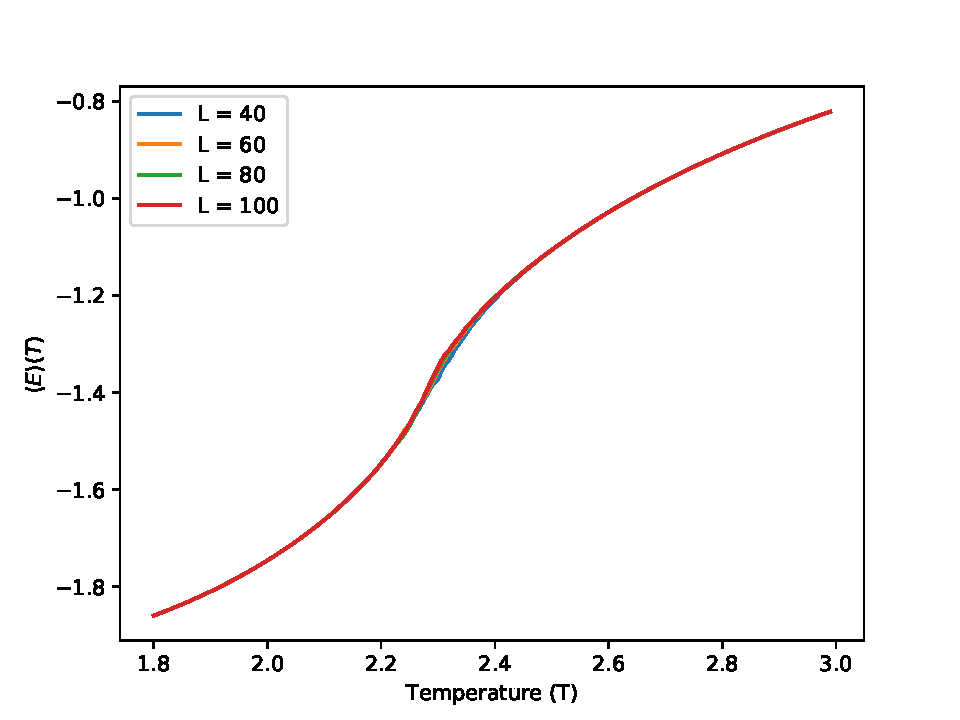
\includegraphics[scale=0.7]{Code_Files/Figures/E_of_T_N_1000000000.pdf}
    \caption{Energy something}
    \label{fig:E_of_T}
\end{figure}
\begin{figure}[H]
    \centering
    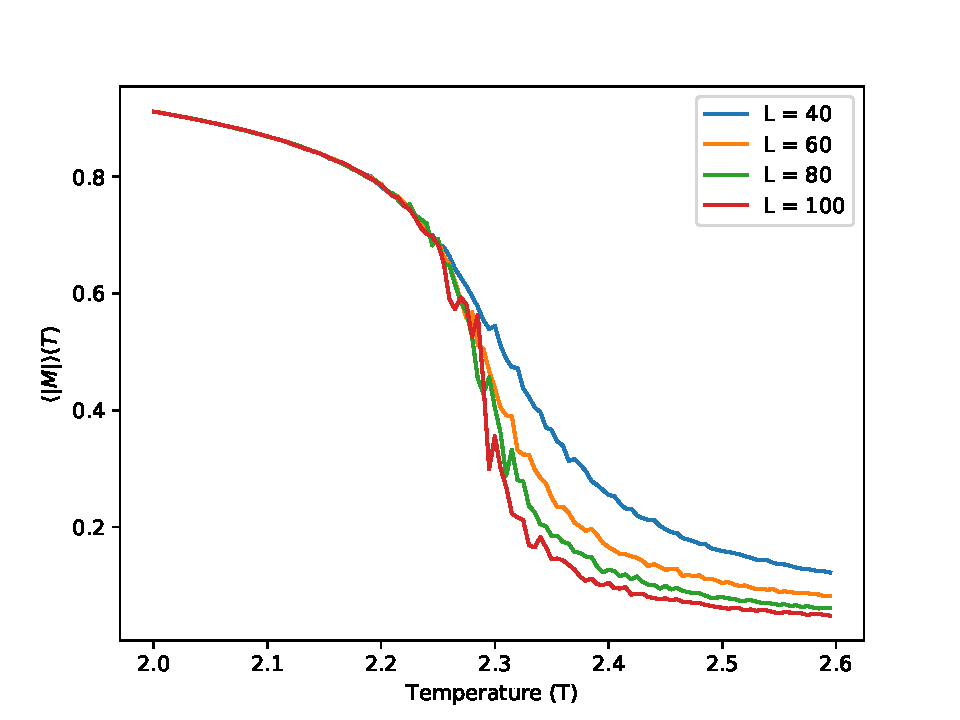
\includegraphics[scale=0.7]{Code_Files/Figures/M_of_T_N_1000000000.pdf}
    \caption{Magnetization something}
    \label{fig:M_of_T}
\end{figure}
\begin{figure}[H]
    \centering
    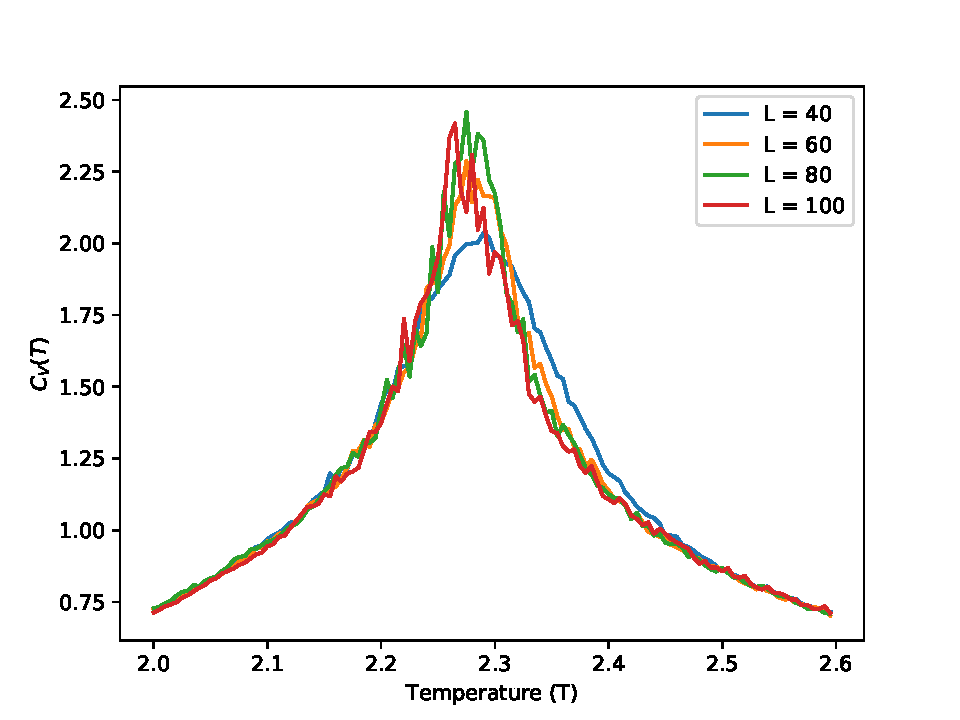
\includegraphics[scale=0.7]{Code_Files/Figures/Cv_of_T_N_1000000000.pdf}
    \caption{Heat capacity something}
    \label{fig:Cv_of_T}
\end{figure}
\begin{figure}[H]
    \centering
    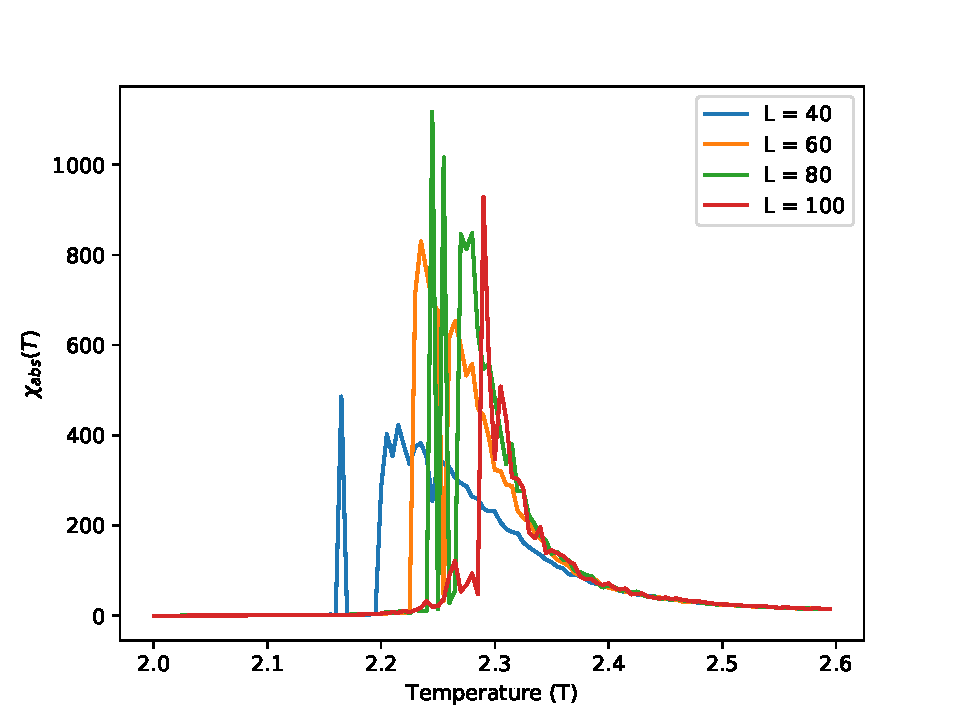
\includegraphics[scale=0.7]{Code_Files/Figures/X_of_T_N_1000000000.pdf}
    \caption{Susceptibility something}
    \label{fig:X_of_T}
\end{figure}


\printbibliography


\end{document}
